%=======================================================================
%  VernaSolver — IEEE Conference Paper
%  How to use in Overleaf:
%    1. Create a new blank project.
%    2. Paste this whole file into main.tex.
%    3. Menu (top-left) → Settings → Compiler → pdfLaTeX.
%    4. Click "Recompile". Done — IEEEtran is built into Overleaf.
%  Everything below (two-column layout, alignment, spacing) is handled
%  automatically by the IEEEtran class — do not change the geometry.
%=======================================================================
\documentclass[conference]{IEEEtran}
\IEEEoverridecommandlockouts

% --- Packages ---------------------------------------------------------
\usepackage{cite}
\usepackage{amsmath,amssymb,amsfonts}
\usepackage{algorithmic}
\usepackage{graphicx}
\usepackage{textcomp}
\usepackage{xcolor}
\usepackage{url}
\usepackage{booktabs}     % nicer tables
\usepackage{listings}     % code listings
\usepackage{tikz}         % native architecture diagram
\usetikzlibrary{shapes.geometric, arrows.meta, positioning, fit, backgrounds}

% --- Fix bad line breaks in URLs --------------------------------------
\def\BibTeX{{\rm B\kern-.05em{\sc i\kern-.025em b}\kern-.08em
    T\kern-.1667em\lower.7ex\hbox{E}\kern-.125emX}}

% --- Listing style for any code snippets ------------------------------
\lstset{
  basicstyle=\ttfamily\footnotesize,
  breaklines=true,
  columns=fullflexible,
  keepspaces=true,
  frame=single,
  framesep=4pt,
  aboveskip=6pt,
  belowskip=6pt
}

\begin{document}

% =====================================================================
%  TITLE
% =====================================================================
\title{VernaSolver: A Retrieval-Augmented Generation System for
Citation-Grounded, Multilingual Question Answering from Academic Textbooks}

% ---------------------------------------------------------------------
%  AUTHORS  (IEEE 3-author block)
% ---------------------------------------------------------------------
\author{
\IEEEauthorblockN{Pritam Bairagi}
\IEEEauthorblockA{\textit{Dept. of Computer Science \& Engineering}\\
\textit{MIT Art, Design and Technology University}\\
Pune, India \\
Enrollment: ADT24SOCB0846}
\and
\IEEEauthorblockN{Shwetaki Killedar}
\IEEEauthorblockA{\textit{Dept. of Computer Science \& Engineering}\\
\textit{MIT Art, Design and Technology University}\\
Pune, India \\
Enrollment: ADT24SOCB1158}
\and
\IEEEauthorblockN{Preksha Pokharna}
\IEEEauthorblockA{\textit{Dept. of Computer Science \& Engineering}\\
\textit{MIT Art, Design and Technology University}\\
Pune, India \\
Enrollment: ADT24SOCB0839}
}

\maketitle

% =====================================================================
%  ABSTRACT
% =====================================================================
\begin{abstract}
AI chatbots like ChatGPT and Claude can answer almost any student
question, but they answer from what they learned during training, not
from the actual textbook a student is studying. Because of this, they
sometimes give wrong answers, make up page numbers, or do not work well
in Indian languages. We built \textit{VernaSolver} to fix this. It is a
study tool that answers questions only from the textbook the student
chooses, and it shows the exact page number for every answer. The
student uploads a textbook as a PDF. Our system reads the text, breaks
it into small parts, turns each part into a numeric form using a small
embedding model, and saves these in a vector database. When a student
asks a question, the system finds the most related parts of the book,
re-checks them with a second model to pick the best ones, and sends
them to an AI model with clear instructions to answer only from those
parts. If the answer is not in the book, the system simply says so
instead of guessing. VernaSolver can also search one book or all books
in a subject, reply in English, Hindi, or Marathi, and create quizzes
and flashcards from the book. In this paper we explain how the system
works, how we keep the answers tied to the book, and how we built it.
\end{abstract}

\begin{IEEEkeywords}
Retrieval-Augmented Generation, Large Language Models, Question
Answering, Vector Database, Semantic Search, Educational Technology,
Multilingual NLP, Citation Grounding.
\end{IEEEkeywords}

% =====================================================================
%  I. INTRODUCTION
% =====================================================================
\section{Introduction}
Today many students use AI chatbots to get help with their studies.
These tools can explain topics and answer questions on almost any
subject. But there is a problem when a student has to study from one
fixed textbook given in their course. A normal chatbot answers from the
huge amount of data it was trained on, not from that exact book. So it
can give an answer that does not match the book, it can make up a page
number that is not real, and it may not follow the syllabus the student
will be tested on. For a student preparing for an exam, an answer that
sounds confident but cannot be checked is not very useful.

There is also a language problem. Many students in India study in Hindi
or Marathi, but most chatbots work best in English. When answers are
both hard to verify and only in English, students cannot fully trust
these tools, even though this is exactly where trust matters the most.

To solve this, we built \textbf{VernaSolver}. The idea behind it is
simple: every answer must come from the student's own textbook, and the
student should be able to check it. VernaSolver uses an approach called
Retrieval-Augmented Generation (RAG)~\cite{lewis2020rag}. In this
approach, instead of letting the AI answer from memory, the system first
finds the most useful parts of the uploaded book and then asks the AI to
answer using only those parts, while showing the page number for each
one.

The main contributions of this work are:
\begin{itemize}
\item A question-answering system that answers only from the chosen
textbook, shows the correct page number, and clearly says when the
answer is not in the book.
\item A search method that combines meaning-based search with a second
checking step, and also rewrites follow-up questions so multi-turn
chats work well.
\item A low-cost design where the heavy search work runs locally on a
normal computer, and the AI model is used only for writing the final
answer, with a backup model in case the main one fails.
\item Extra study features---searching across a full subject, answers in
English, Hindi, and Marathi, and automatic quiz and flashcard
creation---offered through both a command-line tool and a web app.
\end{itemize}

% =====================================================================
%  II. RELATED WORK
% =====================================================================
\section{Related Work}
\textbf{Retrieval-Augmented Generation.} Lewis \textit{et
al.}~\cite{lewis2020rag} introduced RAG, where an AI model is connected
to an outside source of information so it does not have to answer only
from memory. Later studies showed that this way of working reduces wrong
or made-up answers and helps the model point to where the information
came from.

\textbf{Search and re-checking.} Early search methods matched words
directly. Dense passage retrieval~\cite{karpukhin2020dpr} changed this by
comparing meaning instead of just words, which gives better results.
Sentence-BERT~\cite{reimers2019sbert} made it fast to turn short pieces
of text into numbers and compare them. A second model, called a
cross-encoder, can then look at the question and each result together to
pick the best matches.

\textbf{AI models as answer writers.} Modern AI models are good at
reading given text and answering from it. But if they are not clearly
told to use only the given text, they often mix it with what they
already know. This is a problem for exam study, where only the
prescribed book should be used.

VernaSolver is different from a normal RAG chatbot in three ways. It
always shows the page number to the student, it refuses to answer when
the book does not contain the answer, and it is made for studying from a
single textbook in more than one language on a normal computer.

% =====================================================================
%  III. PROBLEM STATEMENT & OBJECTIVES
% =====================================================================
\section{Problem Statement and Objectives}
Normal AI chatbots answer from their training data and not from the
student's actual textbook. This gives answers that cannot be checked,
are sometimes wrong, and often do not support Indian languages. The aim
of this work is to build a system that:
\begin{enumerate}
\item Answers questions using only the textbook the student has chosen,
and does not bring in outside information.
\item Shows the exact page number for every answer, and lets the student
search inside one book or across all books in a subject.
\item Keeps maths steps and figures the same as they are in the book,
instead of the model solving them on its own.
\item Works through two interfaces: a command-line tool for testing and
a web app for normal users.
\end{enumerate}

% =====================================================================
%  IV. SYSTEM ARCHITECTURE
% =====================================================================
\section{System Architecture}
VernaSolver works in three steps: \emph{reading the book},
\emph{searching}, and \emph{answering}. Fig.~\ref{fig:arch} shows how
the data moves through the system.

% ---- Architecture figure (native TikZ — compiles in Overleaf, no image upload) ----
\begin{figure}[!t]
\centering
\resizebox{\columnwidth}{!}{%
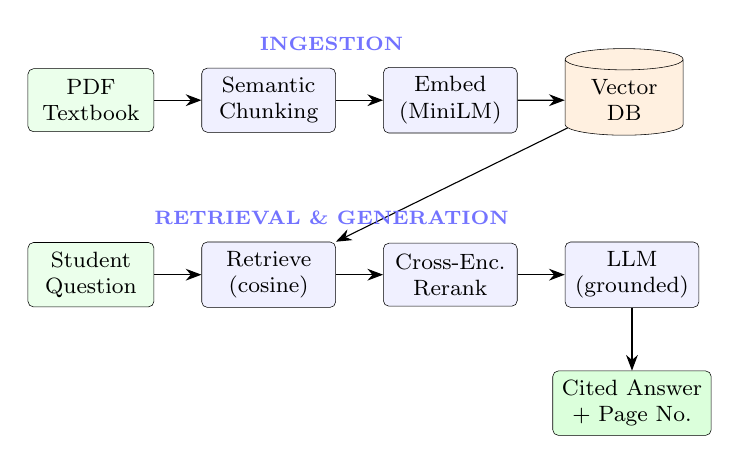
\begin{tikzpicture}[
  node distance=5mm and 6mm,
  font=\footnotesize,
  box/.style={rectangle, rounded corners=2pt, draw=black, very thin,
              minimum height=8mm, minimum width=17mm, align=center,
              fill=blue!6},
  store/.style={cylinder, shape border rotate=90, aspect=0.25, draw=black,
                very thin, minimum height=11mm, minimum width=15mm,
                align=center, fill=orange!12},
  io/.style={rectangle, rounded corners=2pt, draw=black, very thin,
             minimum height=8mm, minimum width=16mm, align=center,
             fill=green!8},
  lbl/.style={midway, font=\scriptsize\itshape, text=black!60},
  arr/.style={-{Stealth[length=2mm]}, thin}
]

% ---- Ingestion row (top) ----
\node[io]    (pdf)   {PDF\\Textbook};
\node[box, right=of pdf]   (chunk) {Semantic\\Chunking};
\node[box, right=of chunk] (embed) {Embed\\(MiniLM)};
\node[store, right=of embed] (db)  {Vector\\DB};

\draw[arr] (pdf)   -- (chunk);
\draw[arr] (chunk) -- (embed);
\draw[arr] (embed) -- (db);

% Ingestion bracket label
\node[font=\scriptsize\bfseries, above=1mm of chunk, xshift=8mm, text=blue!55]
  {INGESTION};

% ---- Query row (bottom) ----
\node[io, below=14mm of pdf] (q) {Student\\Question};
\node[box, right=of q]      (ret)  {Retrieve\\(cosine)};
\node[box, right=of ret]    (rank) {Cross-Enc.\\Rerank};
\node[box, right=of rank]   (llm)  {LLM\\(grounded)};

\draw[arr] (q)   -- (ret);
\draw[arr] (ret) -- (rank);
\draw[arr] (rank)-- (llm);

% DB feeds retrieval
\draw[arr] (db) -- node[lbl, right] {} (ret);

% ---- Output ----
\node[io, below=8mm of llm, fill=green!14] (ans) {Cited Answer\\+ Page No.};
\draw[arr] (llm) -- (ans);

% Query bracket label
\node[font=\scriptsize\bfseries, above=1mm of ret, xshift=8mm, text=blue!55]
  {RETRIEVAL \& GENERATION};

\end{tikzpicture}%
}
\caption{End-to-end VernaSolver RAG pipeline. The ingestion path (top)
converts a PDF into searchable embeddings; the query path (bottom)
retrieves and reranks relevant passages and generates a citation-grounded
answer.}
\label{fig:arch}
\end{figure}

\subsection{Reading the Book}
When a student uploads a PDF, the system reads it page by page using the
PyMuPDF library. Reading it this way keeps track of which text came from
which page, so we can show the right page number later. The text is then
split into small parts of about 400 words each, with a 40-word overlap
between parts. The overlap makes sure that an idea split across two parts
is not lost. Each part is turned into a list of 384 numbers using a small
model called \texttt{all-MiniLM-L6-v2}, which runs on a normal computer
without a graphics card. These numbers, along with the book title,
author, subject, and page number, are saved in a ChromaDB database.

\subsection{Searching}
When a student asks a question, the question is turned into numbers using
the same model and compared with the saved parts of the book to find the
closest matches. These matches are then checked again by a second model
(\texttt{ms-marco-MiniLM-L-6-v2}), which looks at the question and each
match together and picks the best ones. If the student asks a follow-up
like ``explain that more,'' the system uses the earlier chat to rewrite
the question into a full one before searching, so follow-ups work
properly.

\subsection{Answering}
The best matching parts, along with their page numbers, are sent to an AI
model (Anthropic Claude, with OpenAI GPT-4o-mini as a backup). The model
is told to answer using only these parts, to keep maths steps exactly as
written in the book instead of solving them itself, and to say so when
the answer is not there. The answer appears on the screen word by word as
it is written, using a method called Server-Sent Events (SSE). The page
numbers are shown below the answer so the student can check them.

% =====================================================================
%  V. METHODOLOGY
% =====================================================================
\section{How Answers Stay Tied to the Book}
Three things make sure VernaSolver's answers can be trusted.

\textbf{1) Answer only from the book.} The instruction given to the AI
model clearly says it must use only the parts taken from the book, and it
must say the answer is not found when the book does not have it. This
makes the page number a real promise and not just decoration.

\textbf{2) Page number for every answer.} Since each part of the book
keeps its page number all the way through, every answer can be traced
back to a page. The system can even show that page from the PDF with the
used text marked, so the student can see the proof.

\textbf{3) Keep search and writing separate.} The small model on the
computer does all the searching, while the bigger AI model is used only
to write the final answer from text that is already found. This keeps the
cost and waiting time low, and makes sure the AI is reading from the book
instead of answering from memory.

For quizzes and flashcards, the same search step collects the related
text, and the AI model is asked to give its output in a fixed JSON
format. To stop it from writing a normal paragraph instead of JSON, we
start its reply with an opening brace so it has to continue in JSON.

% =====================================================================
%  VI. IMPLEMENTATION
% =====================================================================
\section{Implementation}
VernaSolver is written in Python. Table~\ref{tab:stack} lists the main
tools used. The server side is built with FastAPI and provides web
addresses for chat, managing books, uploading books, making quizzes and
flashcards, and logging in. There is also a command-line tool, built with
Click, that does the same core work and is handy for testing. The web
page is made with plain HTML, CSS, and JavaScript, and shows the answer
as it streams in. User accounts are kept in an SQLite database, with
passwords stored in a safe hashed form (PBKDF2-SHA256) and logins handled
through cookies.

\begin{table}[!t]
\caption{VernaSolver Technology Stack}
\label{tab:stack}
\centering
\renewcommand{\arraystretch}{1.25}
\begin{tabular}{@{}ll@{}}
\toprule
\textbf{Component} & \textbf{Technology} \\
\midrule
Backend framework   & FastAPI (Python) \\
PDF parsing         & PyMuPDF (fitz) \\
Embedding model     & all-MiniLM-L6-v2 (local, CPU) \\
Reranker            & ms-marco-MiniLM-L-6-v2 \\
Vector database     & ChromaDB (persistent) \\
Primary LLM         & Anthropic Claude \\
Fallback LLM        & OpenAI GPT-4o-mini \\
Streaming           & Server-Sent Events (SSE) \\
Authentication      & SQLite + PBKDF2-SHA256 \\
Frontend            & HTML / CSS / JavaScript \\
CLI                 & Click \\
\bottomrule
\end{tabular}
\end{table}

\subsection{Main Settings}
Each part of the book is about 400 words long, with a 40-word overlap and
a minimum of 30 words. The search picks 12 close matches and keeps the
best 5 after the second checking step. The system also remembers up to 6
recent question-and-answer turns for context. These numbers were chosen
to get good search results while not sending too much text to the AI
model at once.

% =====================================================================
%  VII. RESULTS / CURRENT STATUS
% =====================================================================
\section{Current Status and Observations}
We have a working version of the system and have tested it with a few
course textbooks, including \textit{Software Engineering} by Pressman and
\textit{Concepts of Physics} by H.C. Verma. The system answers concept
and definition questions correctly and shows the right page numbers. When
the book does not have the answer, it says so instead of guessing. It can
also make quizzes and flashcards on a chosen topic, and the answers
appear smoothly on screen as they are written. From what we have seen so
far, telling the model to use only the book, along with the second
checking step, keeps the answers close to the book, and rewriting
follow-up questions clearly helps with chats that have more than one
question.

% =====================================================================
%  VIII. LIMITATIONS & FUTURE WORK
% =====================================================================
\section{Limitations and Future Work}
The system depends on how well the text can be read from the PDF. Books
that are only scanned images, without a text layer, are not supported
yet. The search model works best in English, so searching inside Hindi or
Marathi text is weaker, even though the final answer can be given in those
languages. Also, the chat history is kept only in memory, so it is lost
when the server restarts. In the future we plan to add a step that reads
text from scanned books, use a search model that handles Indian languages
better, run proper tests to measure how accurate the answers and page
numbers are, and add limits per user and saved sessions so the system is
ready for real use.

% =====================================================================
%  IX. CONCLUSION
% =====================================================================
\section{Conclusion}
In this paper we presented VernaSolver, a study tool that answers
questions only from the textbook a student picks and shows the page
number for every answer. By doing the search work on a normal computer
and using the AI model only to write the answer from the found text, and
by clearly telling it to stay within the book, the system avoids the
made-up answers and trust problems of normal chatbots. It also adds
support for Indian languages and can create quizzes and flashcards. The
result is a simple, low-cost tool that turns a student's own textbook
into a reliable helper that always backs up its answers with a page
number.

% =====================================================================
%  REFERENCES
% =====================================================================
\begin{thebibliography}{00}

\bibitem{lewis2020rag}
P. Lewis \textit{et al.}, ``Retrieval-augmented generation for
knowledge-intensive NLP tasks,'' in \textit{Advances in Neural
Information Processing Systems (NeurIPS)}, 2020.

\bibitem{karpukhin2020dpr}
V. Karpukhin \textit{et al.}, ``Dense passage retrieval for open-domain
question answering,'' in \textit{Proc. EMNLP}, 2020, pp.~6769--6781.

\bibitem{reimers2019sbert}
N. Reimers and I. Gurevych, ``Sentence-BERT: Sentence embeddings using
Siamese BERT-networks,'' in \textit{Proc. EMNLP-IJCNLP}, 2019,
pp.~3982--3992.

\bibitem{vaswani2017attention}
A. Vaswani \textit{et al.}, ``Attention is all you need,'' in
\textit{Advances in Neural Information Processing Systems (NeurIPS)},
2017.

\bibitem{chromadb}
Chroma, ``ChromaDB: the open-source embedding database,''
\url{https://www.trychroma.com}. (Accessed 2026).

\end{thebibliography}

\end{document}
